\documentclass[
  a4paper,
  11pt,
]{scrartcl}

\usepackage[utf8]{inputenc}
\usepackage[
  %cm,
  headings
]{fullpage}
\usepackage[ngerman]{babel}
\usepackage{amsmath}
\usepackage{amssymb}
\usepackage{amsthm}

\theoremstyle{plain}
\newtheorem{satz}{Satz}
\theoremstyle{definition}
\newtheorem{definition}{Definition}
\theoremstyle{remark}
\newtheorem{beispiel}{Beispiel}

%\usepackage{minted}
\usepackage{listings}
\usepackage{tikz}
\usepackage{pgfplots}
\usepackage{booktabs}
\usepackage{hyperref}

\usepackage[]{algorithm}
\usepackage[]{algorithmic}
\floatname{algorithm}{Algorithmus}

% Für Zeilenumbrüche ohne Indentations
% \setlength{\parindent}{0pt}

% coole Kopf- und Fußzeilen:
\usepackage{fancyhdr}
% Seitenstil ist natürlich fancy:
\pagestyle{fancy}
% alle Felder löschen:
\fancyhf{}

\fancyhead[L]{%
  Seminar: Public-Key-Kryptographie
}
\fancyhead[R]{%
}
%\fancyfoot[L]{}
\fancyfoot[C]{\thepage}

\usepackage{todonotes}

\newcommand{\N}{\mathbb{N}}
\newcommand{\Z}{\mathbb{Z}}
\renewcommand{\P}{\mathbb{P}}
\newcommand{\ggT}{\text{ggT}}
\newcommand{\Mod}[1]{\ \mathrm{mod}\ #1}

\title{Diskrete Logarithmen}

\subtitle{Seminar: Public-Key-Kryptographie}

\author{%
  Martin Darmüntzel \and Hannes Kleinwort
}

\begin{document}

\maketitle

\section{Mathematische Grundlagen}
\label{sec:mathematische_grundlagen}

\begin{definition}[Prime Restklassengruppe]
  Die \emph{prime Restklassengruppe} ist die multiplikative Gruppe der
  Restklassen bezüglich eines Moduls $p$, die zu $p$ teilerfremd sind. Sie wird
  als $\Z_p^*$ notiert.
\end{definition}

Die Bedingung der Teilerfremdheit der einzelnen Elemente $a \in \Z_p^*$ zum
Modul $p$ drückt sich durch $\ggT(a, p) = 1$ für alle $a \in \Z_p^*$ aus. Durch
diese Bedingung und dem Lemma von Bézout hat jedes Element ein multiplikatives
Inverses in $\Z_p^*$. Falls $p$ eine Primzahl ist, dann besteht $\Z_p^*$ aus
der Menge $\left\{1, \ldots, p-1\right\}$, da alle Zahlen aus dieser Menge
teilerfremd zu $p$ sind. Im Allgemeinen ist die Ordnung von $\Z_p^*$ durch die
Eulersche $\varphi$-Funktion bestimmt:
\begin{align*}
  \left| \Z_p^* \right| = \varphi(p)
\end{align*}
Dies ergibt sich direkt aus der Definition der Eulerschen $\varphi$-Funktion.

\begin{definition}[Erzeuger]\label{def:erzeuger}
  Wenn es ein Element $a \in \Z_p^*$ gibt, dessen Potenzen $a^n$ für
  $n \in \Z_p^*$ alle Elemente aus $\Z_p^*$ erzeugt, dann nennt man $a$ einen
  Erzeuger. In $\Z_p^*$ heißen die Erzeuger auch \emph{Primitivwurzeln} modulo
  $p$.
\end{definition}

\begin{beispiel}[Erzeuger]\label{bsp:erzeuger}
  Betrachten wir $\Z_{13}^*$. In dieser Gruppe ist $2$ ein Erzeuger, was man
  durch das Ausrechnen der einzelnen Potenzen überprüfen kann:
  \begin{center}
    \begin{tabular}{r*{12}{r}}
      \toprule
      $x$ & $1$ & $2$ & $3$ & $4$ & $5$ & $6$ & $7$ & $8$ & $9$ & $10$ & $11$ & $12$\\
      \midrule
      $2^x \Mod{13}$ & $2$ & $4$ & $8$ & $3$ & $6$ & $12$ & $11$ & $9$ & $5$ & $10$ & $7$ & $1$\\
      \bottomrule
    \end{tabular}
  \end{center}
  Das Element $3$ ist hingegen kein Erzeuger:
  \begin{center}
    \begin{tabular}{r*{12}{r}}
      \toprule
      $x$ & $1$ & $2$ & $3$ & $4$ & $5$ & $6$ & $7$ & $8$ & $9$ & $10$ & $11$ & $12$\\
      \midrule
      $3^x \Mod{13}$ & $3$ & $9$ & $1$ & $3$ & $9$ & $1$ & $3$ & $9$ & $1$ & $3$ & $9$ & $1$\\
      \bottomrule
    \end{tabular}
  \end{center}
\end{beispiel}

Um herauszufinden, ob ein Element $a \in \Z_p^*$ eine Primitivwurzel ist, müsste
man testen, ob die Potenzen $a^x$ mit $x \in \Z_p^*$ wieder alle Elemente von
$\Z_p^*$ ergeben. Dies ist für große Moduli jedoch sehr aufwändig. Wir können
diesen Test abkürzen, indem wir uns folgende Beobachtung aus
Beispiel~\ref{bsp:erzeuger} zunutze machen: nach dem kleinen Satz von Fermat
muss für jedes Element $a$ aus $\Z_p^*$ die Kongruenz
\begin{align*}
  a^{p-1} \equiv 1 \mod p
\end{align*}
gelten. Für das Element $3 \in \Z_{13}^*$ gilt sie jedoch auch für die
Exponenten $3, 6$ und $9$. Wir müssen demnach nur für bestimmte Exponenten $x$
prüfen, ob $a^x \equiv 1 \mod p$ gilt und falls das der Fall ist, kann $a$ keine
Primitivwurzel sein. Welche Exponenten dies sind, zeigt der folgende Satz.

\begin{satz}\label{satz:primitivwurzeltest}
  Sei $p$ eine Primzahl größer als $2$ und
  $p-1 = q_1^{k_1} \cdot \ldots \cdot q_r^{k_r}$ die Primfaktorzerlegung von
  $p-1$. Eine ganze Zahl $a$ mit $p \nmid a$ ist genau dann Primitivwurzel
  modulo $p$, wenn
  \begin{align*}
    a^{(p-1)/q_i} & \not\equiv 1 \mod p \qquad \text{ für alle } i \in \left\{1, \ldots, r\right\}.
  \end{align*}

  \begin{proof}
    \begin{itemize}
      \item[„$\Rightarrow$“] Durch die Definition der Primitivwurzel modulo $p$
        und dem kleinen Satz von Fermat darf eine Potenz $a^n$ mit
        $n \in \Z_p^*$ nur für den Fall $n = p-1$ kongruent zu $1$ sein. Wäre
        sie es für ein anderes $n$, dann wäre $a$ keine Primitivwurzel.
      \item[„$\Leftarrow$“] Sei $m$ die Ordnung von $a \Mod{p}$ in $\Z_p^*$.
        Nach dem Satz von Lagrange gilt $m \mid (p-1)$. Wenn $m < p-1$ wäre,
        dann müsste es einen Primteiler $q_i \mid (p-1)$ geben, so dass
        $m \mid (p-1)/q_i$, woraus folgt $a^{(p-1)/q_i} \equiv 1 \Mod{p}$. Dies
        ist ein Widerspruch zur Voraussetzung. Demnach hat $a$ die Ordnung
        $m = (p-1)$ und ist Primitivwurzel.
    \end{itemize}
  \end{proof}
\end{satz}

\begin{beispiel}[Primitivwurzel testen]\label{bsp:primitivwurzel_testen}
  Betrachten wir $p = 73 = 2^3 \cdot 3^2 + 1$ und untersuchen mit
  Satz~\ref{satz:primitivwurzeltest}, ob $r_1 = 2, r_2 = 3$ und $r_3 = 5$
  Primitivwurzeln sind.

  \begin{description}
    \item[$r_1 = 2$:]
      \begin{align*}
        2^{72/2}
        & \equiv 2^{36} \equiv 1 \mod p
      \end{align*}
      Damit ist $2$ keine Primitivwurzel.
    \item[$r_2 = 3$:]
      \begin{align*}
        3^{72/2}
        & \equiv 3^{36} \equiv 1 \mod p
      \end{align*}
      Damit ist auch $3$ keine Primitivwurzel.
    \item[$r_3 = 5$:]
      \begin{align*}
        5^{72/2}
        & \equiv 5^{36} \equiv 72 \mod p\\
        5^{72/3}
        & \equiv 5^{24} \equiv 8 \mod p\\
      \end{align*}
      Damit ist $5$ eine Primitivwurzel modulo $73$.
  \end{description}
\end{beispiel}

Mit Satz~\ref{satz:primitivwurzeltest} können wir effizienter eine
Primitivwurzel finden. Wenn wir eine solche gefunden haben, können wir sogar
alle anderen Primitivwurzeln mit dem folgenden Satz bestimmen.

\begin{satz}\label{satz:primitivwurzeln_durch_potenzen}
  Sei $a$ eine Primitivwurzel von $\Z_p^*$. Es ist $a^k$ genau dann eine
  Primitivwurzel von $\Z_p^*$, wenn $k$ und $p-1$ (die Ordnung von $\Z_p^*$)
  teilerfremd sind.

  \begin{proof}
    \begin{itemize}
      \item[„$\Rightarrow$“] Wir setzen $b := a^k$ und nehmen an, dass $k$ und
        $p-1$ teilerfremd sind. Dann gibt es nach dem Lemma von Bézout ganze
        Zahlen $s, t$ mit $s k + t (p-1) = 1$. Daraus folgt
        \begin{align*}
          b^s \equiv a^{k s} \equiv a^{1 - t (p-1)} \equiv a \mod p,
        \end{align*}
        da
        \begin{align*}
          a^{- t (p-1)} \equiv {\left(a^{(p-1)}\right)}^{-t} \equiv 1^{-t} \equiv 1 \mod p
        \end{align*}
        Mittels $b$ kann demnach die Primitivwurzel $a$ erzeugt werden, sodass
        $b$ selbst alle Elemente von $\Z_p^*$ erzeugen kann. Damit ist $b$ eine
        Primitivwurzel.
      \item[„$\Leftarrow$“] Sei wieder $b := a^k$. Wir nehmen an, dass $b$ eine
        Primitivwurzel von $\Z_p^*$ ist. Dann gibt es ein Element
        $s \in \Z_p^*$, so dass $b^s \equiv a \Mod{p}$. Also ist
        $a^{ks} \equiv a \Mod{p}$, woraus $a^{ks - 1} \equiv 1 \Mod{p}$ folgt.
        Demnach muss $ks-1$ ein Vielfaches der Gruppenordnung $p-1$ sein, sodass
        es eine ganze Zahl $t$ mit
        \begin{align*}
          ks - 1 = t(p-1)
        \end{align*}
        geben muss. Dies bedeutet aber, dass $k$ und $p-1$ teilerfremd sein
        müssen.
    \end{itemize}
  \end{proof}
\end{satz}

Da $\Z_p^*$ die Ordnung $\varphi(p) = p-1$ hat und die Anzahl der teilerfremden
Zahlen zu $p-1$ gleich $\varphi(p-1)$ ist, hat $\Z_p^*$ insgesamt
$\varphi(\varphi(p))$ Primitivwurzeln.

\begin{beispiel}[weitere Primitivwurzeln finden]
  Wir betrachten $\Z_{17}^*$ mit dem Erzeuger $3$. Mit
  Satz~\ref{satz:primitivwurzeln_durch_potenzen} wollen wir weitere
  Primitivwurzeln bestimmen.

  Die Menge der zu $p-1 = 16$ teilerfremden Zahlen ist
  \begin{align*}
    \left\{1, 3, 5, 7, 9, 11, 13, 15 \right\}.
  \end{align*}
  Damit erhalten wir die Primitivwurzeln:
  \begin{align*}
    3^1 & \equiv 3 \mod 17\\
    3^3 & \equiv 10 \mod 17\\
    3^5 & \equiv 5 \mod 17\\
    3^7 & \equiv 11 \mod 17\\
    3^9 & \equiv 14 \mod 17\\
    3^{11} & \equiv 7 \mod 17\\
    3^{13} & \equiv 12 \mod 17\\
    3^{15} & \equiv 6 \mod 17\\
  \end{align*}
  Die Menge der Primitivwurzeln von $\Z_{17}^*$ ist somit
  $\left\{ 3, 5, 6, 7, 10, 11, 12, 14 \right\}$.
\end{beispiel}

\begin{definition}[Diskrete Exponentiation, diskreter Logarithmus]
  Sei $g$ ein Erzeuger von $\Z_p^*$. Die diskrete Exponentiation zur Basis $g$
  ist eine Abbildung von $\Z_p^* \to \Z_p^*$ und definiert durch:
  \begin{align*}
    \exp_g: \quad \Z_p^* \to \Z_p^*\\
    x \mapsto g^x
  \end{align*}
  Die dazugehörige Umkehrfunktion
  \begin{align*}
    \log_g: \quad \Z_p^* & \to \Z_p^*\\
    x & \mapsto \log_g x
  \end{align*}
  heißt \emph{diskreter Logarithmus} zur Basis $g$.
\end{definition}

\begin{definition}[Diskretes Logarithmusproblem]\label{def:diskretes_logarithmusproblem}
  Sei $p$ eine Primzahl, $g$ ein Erzeuger von $\Z_p^*$ und $y \in \Z_p^*$.

  Finde ein $x$ mit $1 \leq x \leq p-1$, so dass $g^x \equiv y \mod p$ gilt.
\end{definition}

\section{Anwendung: Ver- und Entschlüsselung}
\label{sec:anwendung_ver_und_entschlusselung}

\section{Berechnung von diskreten Logarithmen}
\label{sec:berechnung_von_diskreten_logarithmen}

\subsection{Naive Berechnung}
\label{sub:naive_berechnung}

Die einfachste Möglichkeit für die Berechnung des diskreten Logarithmus ist das
Durchprobieren. Wir erinnern uns an das diskrete Logarithmusproblem
(Definition~\ref{def:diskretes_logarithmusproblem}): gegeben sei eine Primzahl
$p$, ein Erzeuger $g$ der Gruppe $\Z_p^*$ und ein Element $y$ aus dieser Gruppe.
Wir suchen den Exponenten $x \in \Z_p^*$ für den gilt:
\begin{align*}
  g^x \equiv y \mod p
\end{align*}
Da $\Z_p^*$ nur endlich viele Element enthält, können wir für jedes $x$
überprüfen, ob es die Kongruenz erfüllt.

\begin{algorithm}
  \caption{naiver Berechnungsalgorithmus}
  \begin{algorithmic}
    \REQUIRE{$p \in \P, \left\langle g \right\rangle \in \Z_p^*, y \in \Z_p^*$}
    \FORALL{$x \in \left\{1, \ldots, p-1\right\}$}
      \IF{$g^x \equiv y \mod p$}
        \RETURN{$x$}
      \ELSE{}
        \STATE{$x \leftarrow x + 1$}
      \ENDIF{}
    \ENDFOR{}
  \end{algorithmic}
\end{algorithm}

%\begin{listing}[H]
%  \caption{Implementation des naiven Berechnungsalgorithmus’}
%  \begin{minted}{python}
%    def dlog_naive(root, modulus, value):
%        for x in range(1, modulus):
%            if pow(root, x, modulus) == value:
%                return x
%  \end{minted}
%\end{listing}

\subsection{Pohlig-Hellman-Algorithmus}
\label{sub:pohlig_hellman_algorithmus}

Wenn die Ordnung von $\Z_p^*$ in viele kleine Primfaktoren zerfällt, dann kann
man diesen Umstand zur Berechnung des diskreten Logarithmus nutzen und diese
beschleunigen.

Sei $p-1 = \prod\limits_q q^k$ die Primfaktorzerlegung der Gruppenordnung von
$\Z_p^*$. Zunächst berechnen wir die $q$-ten Einheitswurzeln vom erzeugenden
Element $g$:
\begin{align*}
  r_{q, j} &
    \equiv g^{\frac{j(p-1)}{q}} \mod p &
    \text{ für alle } j = 0, 1, \ldots, q-1
\end{align*}

Wir müssen nun das $x \in \Z_p^*$ finden, für das $g^x \equiv y \mod p$ gilt.
Mit der Primfaktorzerlegung von $p-1$ brauchen wir nur $x \Mod{q^k}$ für jeden
Primfaktor $q$ von $p-1$ zu bestimmen, da sich $x$ dann aus dem Chinesischen
Restsatz ergibt. Wir fixieren jetzt einen Primfaktor $q$ von $p-1$ und zeigen,
wie sich daraus die Kongruenz $x \Mod{q^k}$ ergibt.

Angenommen
\begin{align*}
  x & \equiv x_0 + x_1 q + \cdots + x_{k-1} q^{k-1} \mod q^k
    & \text{ mit } 0 \leq x_i < q
\end{align*}
Für $x_0$ berechnen wir $y^{\frac{p-1}{q}}$. Da $y^{p-1} \equiv 1 \Mod{p}$,
erhalten wir eine $q$-te Wurzel von $1$. Aus $y = g^x$ folgt
\begin{align*}
  y^{\frac{p-1}{q}} &
    = g^{\frac{x(p-1)}{q}}
    = g^{\frac{x_0 (p-1)}{q}}
    = r_{q, x_0}
\end{align*}
Also vergleichen wir $y^{\frac{p-1}{q}}$ mit den zuvor berechneten Wurzeln
$r_{q, j}$ und setzen $x_0$ auf den Wert von $j$ für den
$y^{\frac{p-1}{q}} = r_{q, j}$ gilt.

Um danach $x_1$ zu finden, ersetzen wir $y$ durch $y_1 = \frac{y}{g^{x_0}}$,
denn $y_1$ hat dann den disk. Logarithmus
\begin{align*}
  x - x_0 \equiv x_1 q + \cdots + x_{k-1} q^{k-1} \mod q^k
\end{align*}
Da $y_1$ eine Potenz von $q$ ist, erhalten wir
$y_1^{\frac{p-1}{q}} \equiv 1 \Mod{p}$ und
\begin{align*}
  y_1^{\frac{p-1}{q^2}} &
    = g^{\frac{(x-x_0) (p-1)}{q^2}}
    = g^{\frac{(x_1 + x_2 q + \cdots) (p-1)}{q}}
    = g^{\frac{x_1 (p-1)}{q}}
    = r_{q, x_1}.
\end{align*}
Also vergleichen wir $y_1^{\frac{p-1}{q^2}}$ mit den berechneten Wurzeln
$r_{q, j}$ und setzen $x_1$ auf den Wert von $j$ für den
$y_1^{\frac{p-1}{q^2}} = r_{q, j}$ gilt.

Dieses Verfahren setzen wir induktiv fort. Für jedes $i = 1, 2, \ldots, k-1$
setzen wir
\begin{align*}
  y_i & = \frac{y}{g^{x_0 + x_1 q + \cdots x_{i-1} q^{i-1}}}.
\end{align*}
Dieses $y_i$ hat den disk. Logarithmus
$x_i q^i + \cdots + x_{k-1} q^{k-1} \Mod{q^k}$. Da $y_i$ eine Potenz von $q^i$
ist, erhalten wir $y_i^{(p-1)/q^i} \equiv 1$ und
\begin{align*}
  y_i^{\frac{p-1}{q^{i+1}}} &
    = g^{\frac{(x_i + x_{i+1} q + \cdots) (p-1)}{q}}
    = g^{\frac{x_i (p-1)}{q}}
    = r_{q, x_i}
\end{align*}
Wir setzen $x_i$ auf den Wert von $j$ für den
$y_i^{\frac{p-1}{q^{i+1}}} = r_{q, j}$ ist.

Abschließend erhalten wir die Kongruenz $x \Mod{q^k}$. Wenn wir dieses Verfahren
für jeden Primfaktor von $p-1$ durchgeführt haben, nutzen wir den Chinesischen
Restsatz um $x$ zu bestimmen.


\subsection{Komplexität Naiver Algorithmus}
\label{sub:komplexitaet_naiver_algorithmus}

Zur Berechnung des diskreten Logarithmus $\text{DL}(y,g,p) = x$ als Lösung der Gleichung\\
$g^x \equiv y \mod p$ ist kein effizientes Verfahren bekannt. Alle bekannten
Verfahren beruhen im Grunde auf einer Brute-Force-Suche über die Menge der
möglichen Lösungen $\Z_p^* = \{1, 2, \ldots, p-1\}$ mit der Komplexität
$\mathcal{O}(p)$.
Wenn man die Komplexität über die Bitlänge $n$ der Primzahl $p$ darstellt, mit
$n = \left\lfloor \log_2 p \right\rfloor + 1 \approx \log_2 p$, so ergibt sich
exponentielle Komplexität $\mathcal{O}(2^n)$. Dazu ein Rechenbeispiel:

\begin{beispiel}
  Angenommen man sucht mit dem naiven Algorithmus die Lösung $x$ zur Eingabe
  $(y, g, p)$, d.\,h. man probiert alle möglichen Lösungen aus $\Z_p^*$ durch,
  bis man die Lösung gefunden hat. Zusätzlich stehen einem dazu die
  Rechenleistung von einer Anzahl von $10^{10}$ Prozessoren zur Verfügung,
  welche jeweils mit einer Frequenz von $10 \text{\,GHz}$ ($= 10^{10} \cdot s^{-1}$)
  operieren und jeweils mit jedem Berechnungsschritt eine modulare Potenz, also
  die Funktion $f(x, g, p) = g^x \mod p$, berechnen können. Dann hätte man eine
  Rechenleistung von $10^{20}$ modularen Potenzen pro Sekunde. Mit
  $10^{20} \leq 2^{67}$ ergibt sich die Zeit $t$ zur Berechnung aller modularen
  Potenzen von allen möglichen Lösungen aus $\Z_p^*$ zu
  $t \geq \frac{2^n}{2^{67}\cdot s^{-1}}=2^{n-67} s$. Jetzt kann man leicht die
  Primzahl $p$ bzw. deren Bitlänge $n$ so groß setzen, dass die Zeit $t$ größer
  wird als das Alter des Universums:
  \begin{align*}
    t_{\text{Alter des Universums}} & = 14 \cdot 10^9 y\\
    & = 14 \cdot 10^9 \cdot 365 \cdot 24 \cdot 60\cdot 60\cdot s\\
    & \leq 2^{59}\cdot s\\
    t_{\text{Alter des Universums}} \leq 2^{59}\cdot s & \leq 2^{n-67}\cdot s \leq t\\
    59 & \leq n-67\\
    n & \geq 59+67\\
    n & \geq 126
  \end{align*}
  Für eine Primzahl $p$ mit einer Bitlänge $n \geq 126$ dauert die Berechnung
  aller möglichen modularen Potenzen mit der oben genannten Hardware also länger
  als das Universum alt ist. Selbst wenn man annimmt, dass im Mittel die Lösung
  mit dem naiven Algorithmus nach der Hälfte der Rechenschritte gefunden wird,
  ist diese Zeitspanne unrealistisch. Außerdem kann, z.\,B. bei Verwendung des
  Diskreten-Logarithmus-Problems in der Verschlüsselung, jede
  nicht-exponentielle Verbesserung des Algorithmus durch eine kostengünstige
  Vergrößerung der Bitlänge $n$ der Primzahl $p$ ausgeglichen werden. Sollte
  sich z.\,B. die gegebene Rechenleistung um den Faktor $x$ vergrößern, so
  müsste die Bitlänge $n$ der Primzahl $p$ lediglich um den Betrag
  $d = \left\lfloor \log_2 x \right\rfloor + 1$ vergrößert werden:
  $n_{\text{neu}} = n_{\text{alt}} + d$. Würde die Rechenleistung sich also
  z.\,B. verzehnfachen, wäre also $x=10$, so würde eine konstante Vergrößerung
  der Bitlänge von $d=4$ dies wieder ausgleichen.
\end{beispiel}

\subsection{Diffie-Hellman-Merkle Schlüsselaustausch (DHKE)}
\label{sub:diffie_hellman_key_exchange}

Der auf der Schwierigkeit des Diskreten-Logarithmus-Problems beruhende Diffie-Hellman-Merkle Schlüsselaustausch, englisch: \textbf{D}iffie-\textbf{H}ellman-\textbf{K}ey-\textbf{E}xchange (\textbf{DHKE}), hat den folgenden Ablauf:
Zwei Kommunikationspartner, hier Alice und Bob, kommunizieren über einen unsicheren Kanal und wollen einen Schlüssel für eine sichere Kommunikation, z.B. durch eine symmetrische Verschlüsselung, austauschen.

Im ersten Schritt wählt Alice eine ausreichend große und den \todo{bekannte Schwachstellen rausnehmen?}bekannten Schwachstellen des Verfahrens ausweichende Primzahl $p$, mit $p = 2 \cdot q + 1$, $q$ prim. Ausreichend groß bedeutet hierbei, dass die Bitlänge $n$ der Primzahl $p$ so groß ist, dass die Berechnung des diskreten Logarithmus $\text{DL}(y,g,p)$ mit bekannten Algorithmen und aktueller Hardware auf absehbare Zeit nicht möglich sein wird (siehe Abschnitt  \ref{sub:komplexitaet_naiver_algorithmus}). Weiterhin sucht Alice einen \todo{ist die Formulierung bei Erzeuger korrekt?}Erzeuger $g \in \Z_p^*$, $\Z_p^* = \{1, 2, \ldots, p-1\}$, welcher $g^k \mod p$, $k \in \N \backslash \{0\}$, zyklisch ohne Untergruppen auf $\Z_p^*$ abbildet (siehe Abschnitt  \ref{def:erzeuger}). Dann wählt Alice ihren geheimen privaten Schlüssel $a \in \Z_p^*$,  berechnet ihren öffentlichen Schlüssel $A$ mit $A \equiv g^a \mod p$ und sendet ($g$, $p$, $A$) über den unsicheren Kanal an Bob.

Im zweiten Schritt wählt Bob seinen geheimen privaten Schlüssel $b \in \Z_p^*$, berechnet seinen öffentlichen Schlüssel $B$ mit $B \equiv g^b \mod p$ und sendet $B$ über den unsicheren Kanal an Alice.
Der gemeinsame geheime Schlüssel $K$ ergibt sich nun auf der Seite von Alice mit
\begin{align*}
	K \equiv B^a \mod p
\end{align*}
und auf der Seite von Bob mit
\begin{align*}
	K \equiv A^b \mod p \text{.}
\end{align*}

\begin{figure}[!htb]
  \centering
  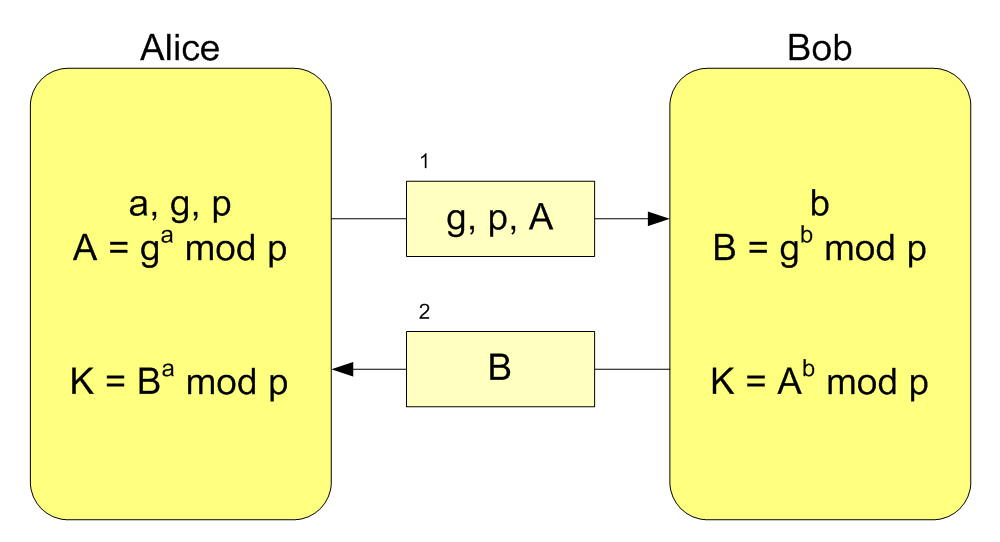
\includegraphics[width=\textwidth]{Diffie-Hellman-Schluesselaustausch2.png}
  \caption{Diffie-Hellman-Merkle-Schlüsselaustausch}
  \label{fig:dhke}
\end{figure}

\subsubsection{Korrektheit: Diffie-Hellman-Merkle Schlüsselaustausch (DHKE)}
\label{sub:proof_dhke}
Zur Korrektheit des Diffie-Hellman-Merkle Schlüsselaustausches: Beide Kommunikationspartner haben den gleichen Schlüssel $K = K_1 = K_2$:
\begin{proof}
Es gilt \todo{quelle einfügen [Menezes, S.68 2.112(V)]}, wenn \todo{Satz in mathematische grundlagen einfügen? }
\begin{align*}
a & \equiv a_1 \mod n
\end{align*}
und
\begin{align*}
b & \equiv b_1 \mod n \text{,}\\
n & \in \N \backslash \{0\}
\end{align*}
dann folgt daraus
\begin{align*}
a \cdot b & \equiv a_1 \cdot b_1 \mod n \text{.}
\end{align*}
Nimmt man jetzt an, dass $a=b$ also
\begin{align*}
a \cdot a & \equiv a_1 \cdot a_1 \mod n
\end{align*}
dann folgt
\begin{align*}
a^k & \equiv a_1^k \mod n \text{,}\\
k & \in \N \backslash \{0\}
\end{align*}
und daraus
\begin{align*}
(a^k)^u & \equiv (a_1^k)^u \mod n \text{,}\\
u & \in \N \backslash \{0\}\text{,}
\end{align*}
womit sich ergibt, dass
\begin{align*}
(a_1^k \mod n)^u & \equiv (a_1^k)^u \mod n
\end{align*}
und
\begin{align*}
(a_1^k \mod n)^u & \equiv a_1^{k\cdot u} \mod n \text{.}
\end{align*}
Mit dieser Kongruenz lässt sich nun einfach zeigen, dass die Schlüssel $K_1$ von Alice und $K_2$ von Bob kongruent sind:
\begin{align*}
K_1 & \equiv B^a \mod p\\
& \equiv (g^b)^a \mod p\\
& \equiv g^{b \cdot a} \mod p\\
& \equiv g^{a \cdot b} \mod p\\
& \equiv (g^a)^b \mod p\\
& \equiv A^b \mod p\\
& \equiv K_2
\end{align*}
\end{proof}

\begin{beispiel}\label{bsp:dhke}

\end{beispiel}

\end{document}
